\begin{figure}[!ht]
    \centering
    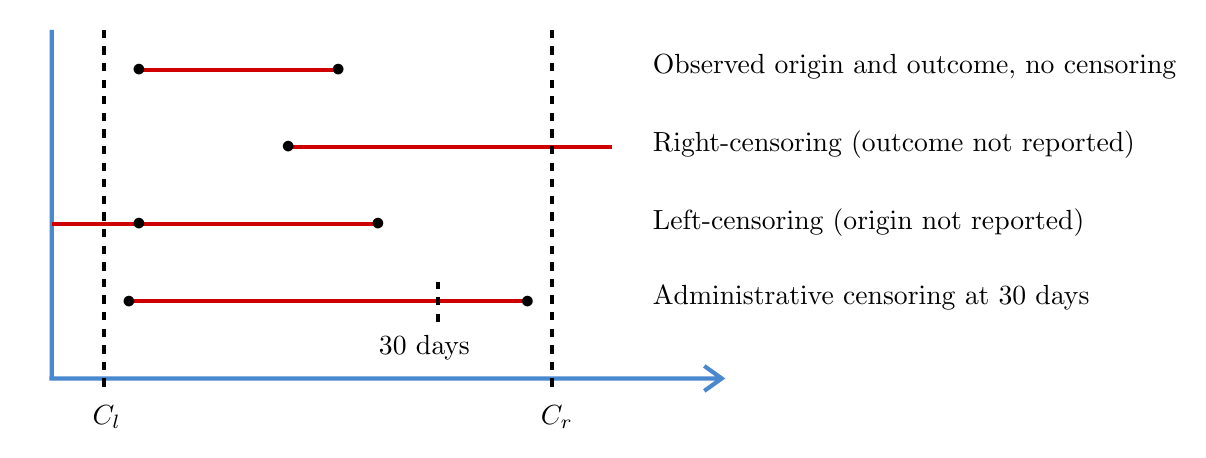
\begin{tikzpicture}[x=0.9pt,y=0.9pt,yscale=-1,xscale=1]
        \path (70,230); %set diagram left start at 0, and has height of 200

        %Shape: Axis 2D [id:dp048941842347560494] 
        \draw [color={rgb, 255:red, 73; green, 135; blue, 206 }, draw opacity=1 ][line width=1.5][-]
        % axes
        (78.67,210.33) -- (348.67,210.33)
        (79.67,70.33) -- (79.67,210.33)

        % arrow
        (341.67,205.33) -- (348.67,210.33) -- (341.67,215.33);

        \draw;

        \draw [color={rgb, 255:red, 206; green, 0; blue, 0 }, draw opacity=1][line width=1.5][-]

        (110.67,179.33) -- (270.67,179.33)
        (79.67,148.33) -- (210.67,148.33)
        (174.67,117.33) -- (304.67,117.33)
        (114.67,86.33) -- (194.67,86.33);

        \draw;

        \draw [color={rgb, 255:red, 0; green, 0; blue, 0 }, draw opacity=1][line width=1.5][-][dashed]
        (280.67,70.33) -- (280.67,215.33)
        (100.67,70.33) -- (100.67,215.33)
        (234.67,187.66) -- (234.67,171.66);
        \draw;

        \draw [-] (95,220) node [anchor=north west][inner sep=0.75pt] [align=left] {$C_l$};
        \draw [-] (275,220) node [anchor=north west][inner sep=0.75pt] [align=left] {$C_r$};

        \draw [-] (320,79) node [anchor=north west][inner sep=0.75pt] [align=left] {Observed origin and outcome, no censoring};
        \draw [-] (320,110) node [anchor=north west][inner sep=0.75pt] [align=left] {Right-censoring (outcome not reported)};
        \draw [-] (320,141) node [anchor=north west][inner sep=0.75pt] [align=left] {Left-censoring (origin not reported)};
        \draw [-] (320,172) node [anchor=north west][inner sep=0.75pt] [align=left] {Administrative censoring at 30 days};

        \draw [-] (210,192) node [anchor=north west][inner sep=0.75pt] [align=left] {30 days};

        % dots
        \foreach \Point in {
                (110.67,179.66),
                (270.67,179.66),
                (174.67,117.66),
                (114.67,148.66),
                (210.67,148.66),
                (114.67,86.66),
                (194.67,86.66)}{
                \node at \Point {$\bullet$};
            }

    \end{tikzpicture}
    \caption[Examples of right, left, and administrative censoring for patients in time-to-event data with origin and outcome information reported]{Examples of right, left, and administrative censoring for patients in time-to-event data with origin and outcome information reported. $C_l$: left-censoring time, $C_r$: right-censoring time, $\bullet$: reported origin, outcome, or intermediate event.}\label{fig:censoring}
\end{figure}